\documentclass[brazilian, fleqn]{article}

\usepackage{babel}
\usepackage[utf8]{inputenc}
\usepackage[T1]{fontenc}
\usepackage{lmodern}

\usepackage{amssymb,amsfonts,amsmath}

\usepackage{tikz}
\usetikzlibrary{calc}

\usepackage[left=2cm, bottom=2cm, right=1.5cm, top=1.5cm]{geometry}

\usepackage{siunitx}
\sisetup{locale = FR}

\usepackage{tcolorbox}
\tcbuselibrary{skins}
\tcbset{boxrule=0pt, top=0pt, bottom=0pt, skin=bicolor, interior style={left color=black!10}}

\DeclareMathOperator{\sen}{sen}
\DeclareMathOperator{\tg}{tg}

\begin{document}
\section*{\centering Questão de aluno 14/04/2023}

\begin{center}
    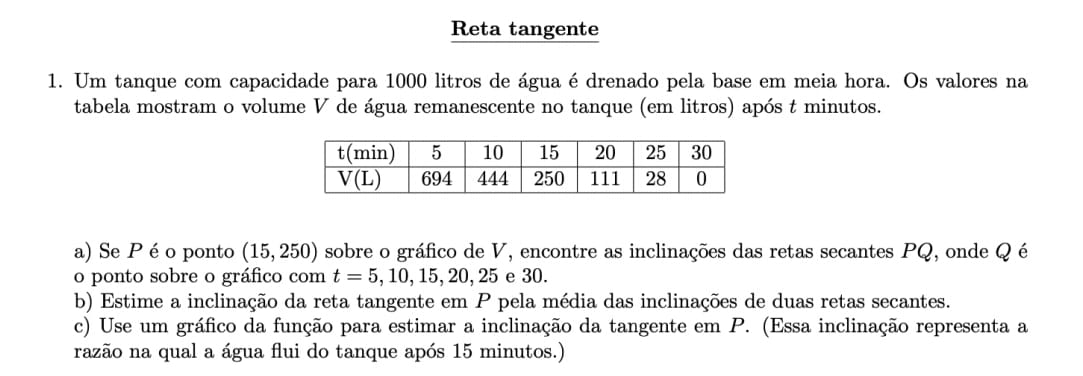
\includegraphics[width=\textwidth]{quest-1.jpg}
\end{center}

\textit{Solução}:\\
a)
\[
    m=\frac{y_Q-y_P}{x_Q-x_P}=
    \begin{cases}
        \dfrac{694-250}{5-15}=\num{-44.40}\\ \\
        \dfrac{444-250}{10-15}=\num{-38.80}\\ \\
        \dfrac{250-250}{15-15}=\text{indeterminado pois P=Q e somente 
        temos secante com dois pontos diferentes} \\ \\
        \dfrac{111-250}{20-15}=\num{-27.80}\\ \\
        \dfrac{28-250}{25-15}=\num{-22.20}\\ \\
        \dfrac{0-250}{30-15}=\num{-16.67}
    \end{cases}
\]

b)
\[
    m_{\text{médio}} = \frac{\num{-38.8}-\num{27.8}}{2}=\num{-33.3}{2}
\]

c)
\begin{center}
    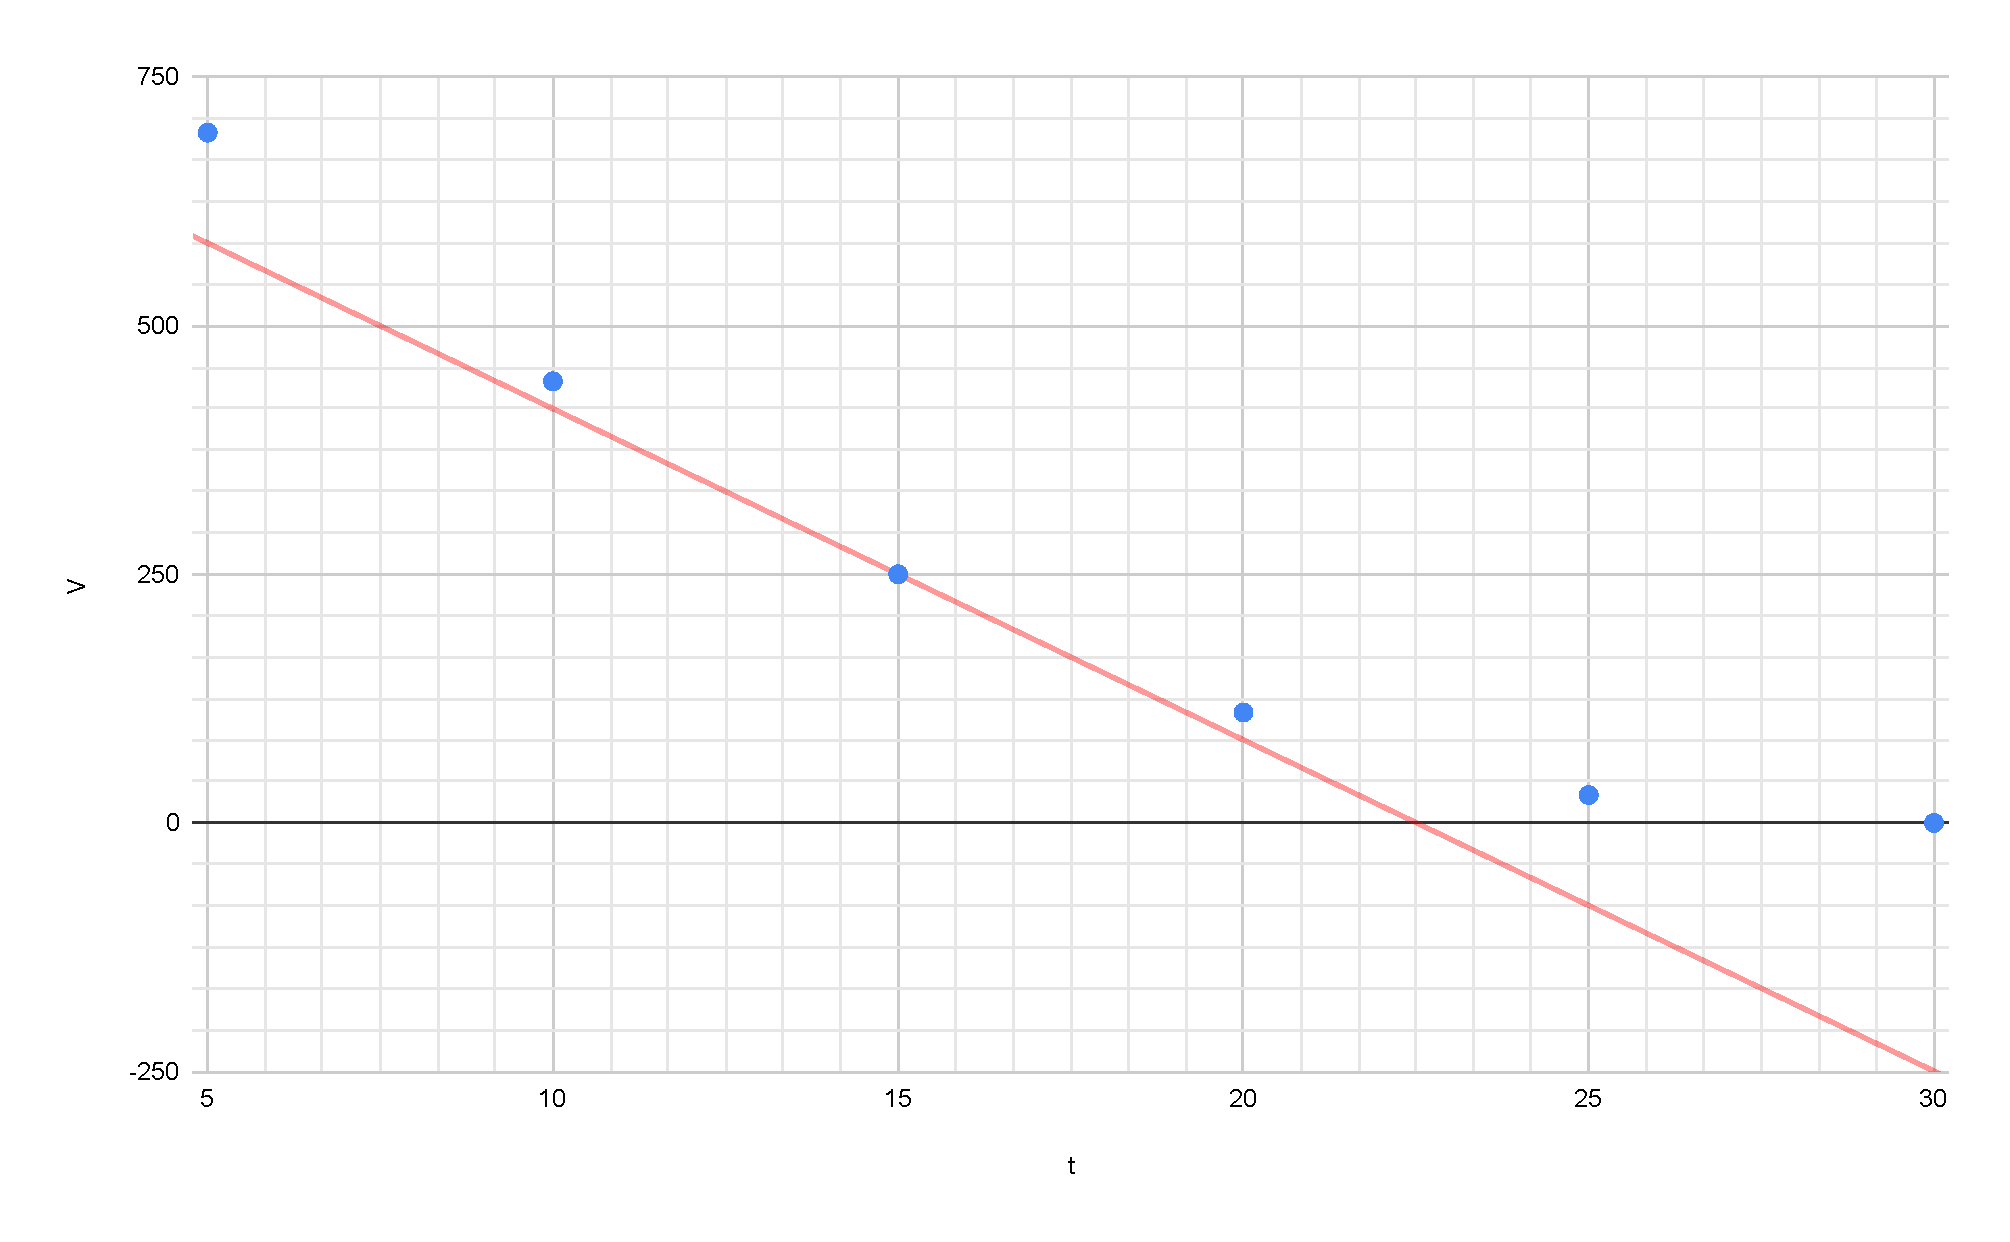
\includegraphics[width=\textwidth]{chart.pdf}
\end{center}
A linha vermelha é a \textit{melhor} reta tangente que pode ser desenhada
sem ''encostar'' nos outros pontos. Para determinar a inclinação dessa reta
usamos os pontos 
\(M\left(5+3\times \dfrac{5}{6},500\right)\) e 
\(N\left(15+3\times\dfrac{5}{6},4\times\dfrac{250}{6}\right)\),
obtidos do gráfico com o auxílio das divisões horizontais e verticais da ''folha''

Assim, temos que a inclinação da reta tangente desenhada é dada por 
\[
    m = \frac{4\times\dfrac{250}{6}-500}
    {15+3\times\dfrac{5}{6}-\left(5+3\times \dfrac{5}{6}\right)} = 
    -\frac{100}{3}=\num{-33.33}\ldots
\]
\end{document}
